\subsection*{Partie I. Flocons de Von Koch}
\begin{enumerate}
 \item Procédures \verb|a(E)| , \verb|l(E)| , \verb|r(E)|.
\begin{verbatim}
from math import cos, sin, pi

def a(E):
    plt.plot([E[2],E[2]+E[0]],[E[3],E[3]+E[1]],'g')
    return [E[0],E[1],E[2]+E[0],E[3]+E[1]]
    
def l(E):
    return [cos(alpha)*E[0] - sin(alpha)*E[1], 
            sin(alpha)*E[0] + cos(alpha)*E[1], E[2], E[3]]

def r(E):
    return [cos(alpha)*E[0] + sin(alpha)*E[1],
            -sin(alpha)*E[0] + cos(alpha)*E[1], E[2], E[3]]
    
func_dic = {'a':a, 'l':l, 'r':r}
\end{verbatim}
Noter que les lignes de code ont été coupées pour la présentation.
\item \begin{enumerate}
 \item La chaîne qui correspond au triangle équilatéral initiateur est \verb|allalla|.
\item La chaîne qui pour le motif est \verb|arallara|.
\end{enumerate}

\item La procédure d'affichage est :
\begin{verbatim}
def affiche(L):
    plt.clf()
    plt.figure(1)
    plt.axis('equal')
    plt.axis('off')
    E = [1.,0.,0.,0.]
    for lettre in L:
        E = func_dic[lettre](E)
\end{verbatim}

\begin{figure}
 \centering
 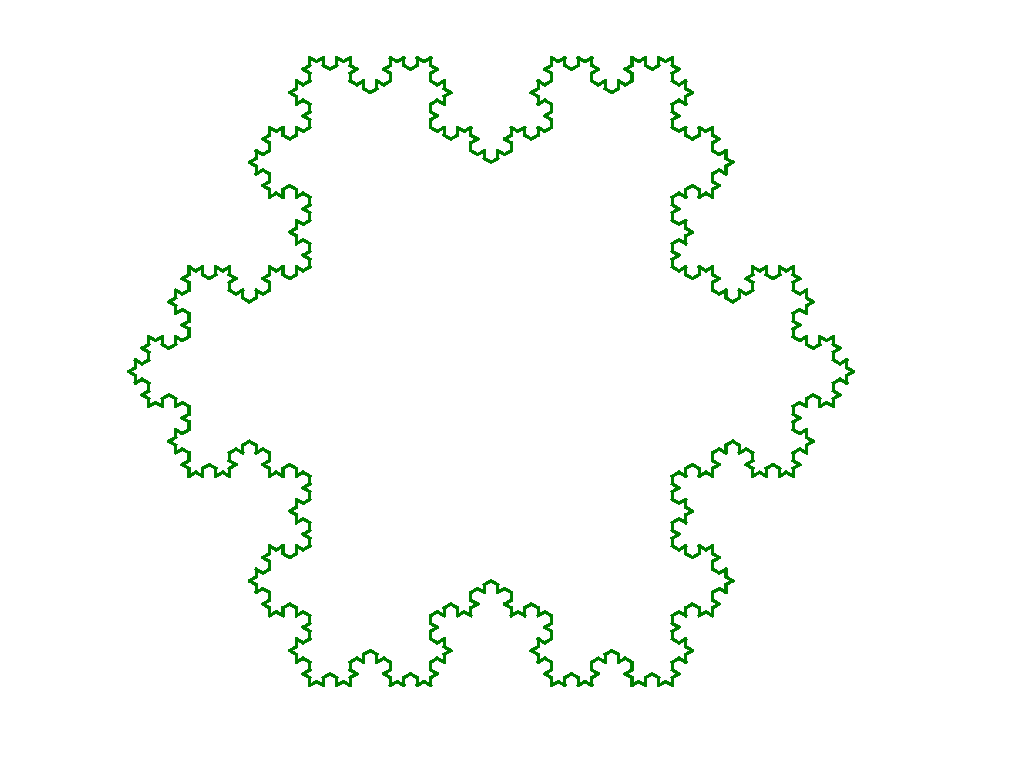
\includegraphics[width=6cm]{Creecriture_1_fig.pdf}
 \caption{Le flocon après 4 itérations}
 \label{fig:Creecriture_1}
\end{figure}

\item Formons une boucle pour pouvoir choisir le nombre de fois où on effectue la substitution. Le dessin obtenu est en figure \ref{fig:Creecriture_1}.
\begin{verbatim}
init = "allalla"
motif = "arallara"
alpha = pi/3

texte  = init
for i in range(4):
    texte = texte.replace('a',motif)

affiche(texte)
\end{verbatim}

\end{enumerate}

\subsection*{Partie II. Dessins de plantes}
\begin{enumerate}
 \item Réécritures des procédures \verb|a(lE)| , \verb|l(lE)| , \verb|r(lE)|.
\begin{verbatim}
def a(lE):
    n = len(lE)-1
    E = lE[n] # état actuel
    plt.plot([E[2],E[2]+E[0]],[E[3],E[3]+E[1]],'g')
    lE[n] = [E[0],E[1],E[2]+E[0],E[3]+E[1]] 
    return lE
    
def l(lE):
    n = len(lE)-1
    E = lE[n] # état actuel
    lE[n] = [cos(alpha)*E[0] - sin(alpha)*E[1],
             sin(alpha)*E[0] + cos(alpha)*E[1], E[2], E[3]]
    return lE

def r(lE):
    n = len(lE)-1
    E = lE[n] # état actuel
    lE[n] = [cos(alpha)*E[0] + sin(alpha)*E[1],
            -sin(alpha)*E[0] + cos(alpha)*E[1], E[2], E[3]]
    return lE
\end{verbatim}

\item Procédure \verb|e(lE)| et \verb|m(lE)|.
\begin{verbatim}
def e(lE):
    n = len(lE)-1
    E = lE[n] # état actuel
    lE.append(E)
    return lE

def m(lE):
    lE.pop()
    return lE
    
func_dic = {'a':a, 'l':l, 'r':r, '(':e, ')':m}
\end{verbatim}

\item Réécriture de \verb|affiche(L)|. Très peu de modifications à effectuer.
\begin{verbatim}
def affiche(L):
    plt.clf()
    plt.figure(1)
    plt.axis('equal')
    plt.axis('off')
    lE = [[0.,1.,0.,0.]]
    for lettre in L:
        lE = func_dic[lettre](lE)
\end{verbatim}
\begin{figure}
   \centering
   \begin{subfigure}[b]{6cm}
     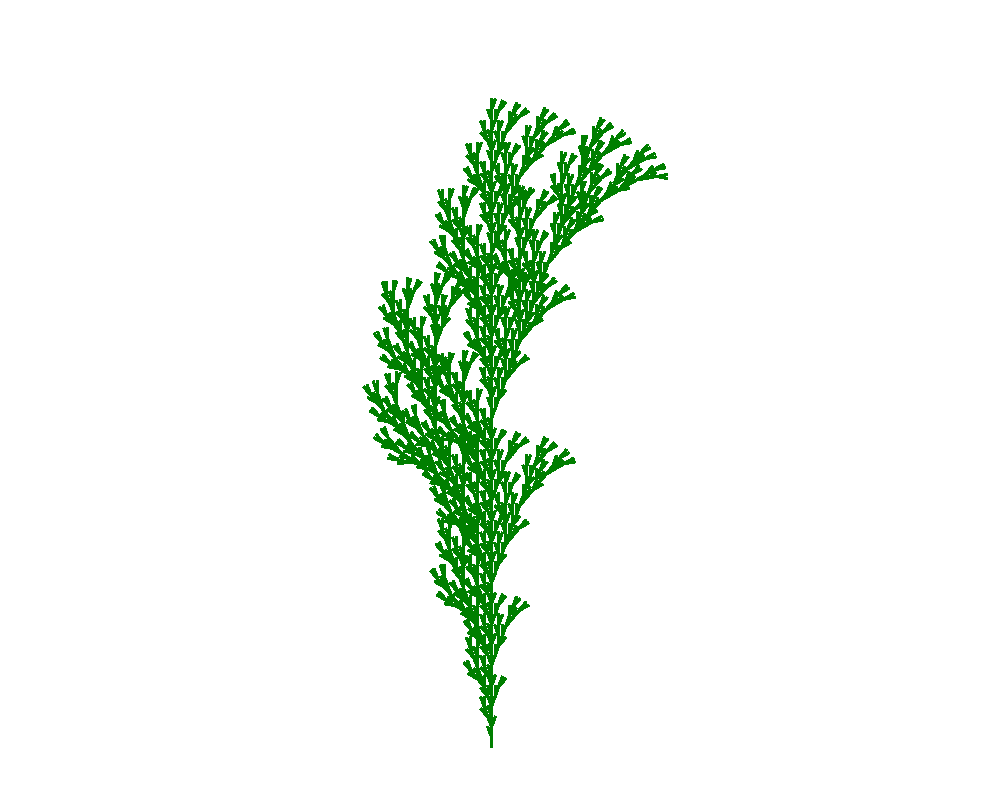
\includegraphics[width=6cm]{Creecriture_2_fig.pdf}
     \caption{"a(la)a(ra)(a)" 5 itér.}
     \label{fig:Creecriture_2}
    \end{subfigure}
  \begin{subfigure}[b]{6cm}
    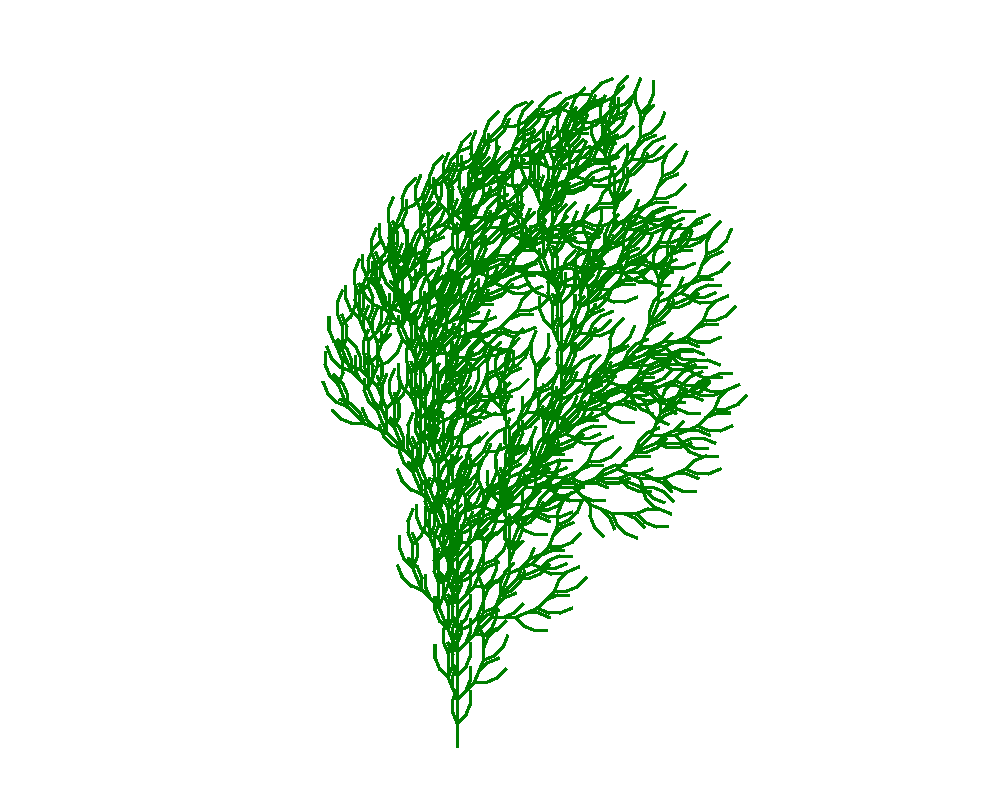
\includegraphics[width=6cm]{Creecriture_3_fig.pdf}
    \caption{"aar(ralala)l(larara)" 4 itér.}
    \label{fig:Creecriture_3}
   \end{subfigure}
   \caption{Modèles sans apex}
\end{figure}

\item On procède avec les exemples comme avec le flocon. Le premier exemple donne le dessin de l'énoncé. Le deuxième est en figure \ref{fig:Creecriture_2} et le troisième en figure \ref{fig:Creecriture_3}.
\item Les apex n'interviennent que pour les substitutions, il faut bien veiller à substituer à la fois  pour \verb|a| et pour \verb|x|. En ce qui concerne \verb|affiche|, rien n'est à changer mais des appels \verb|x(lE)| sont effectuer. Il faut donc écrire une procédure \verb|x(lE)| qui renvoie \verb|lE| sans le modifier et ne pas oublier de l'insérer dans le dictionnaire.
\begin{verbatim}
def x(lE):
  return lE
end proc:
\end{verbatim}
\end{enumerate}
\begin{figure}
  \centering
  \begin{subfigure}[b]{4cm}
    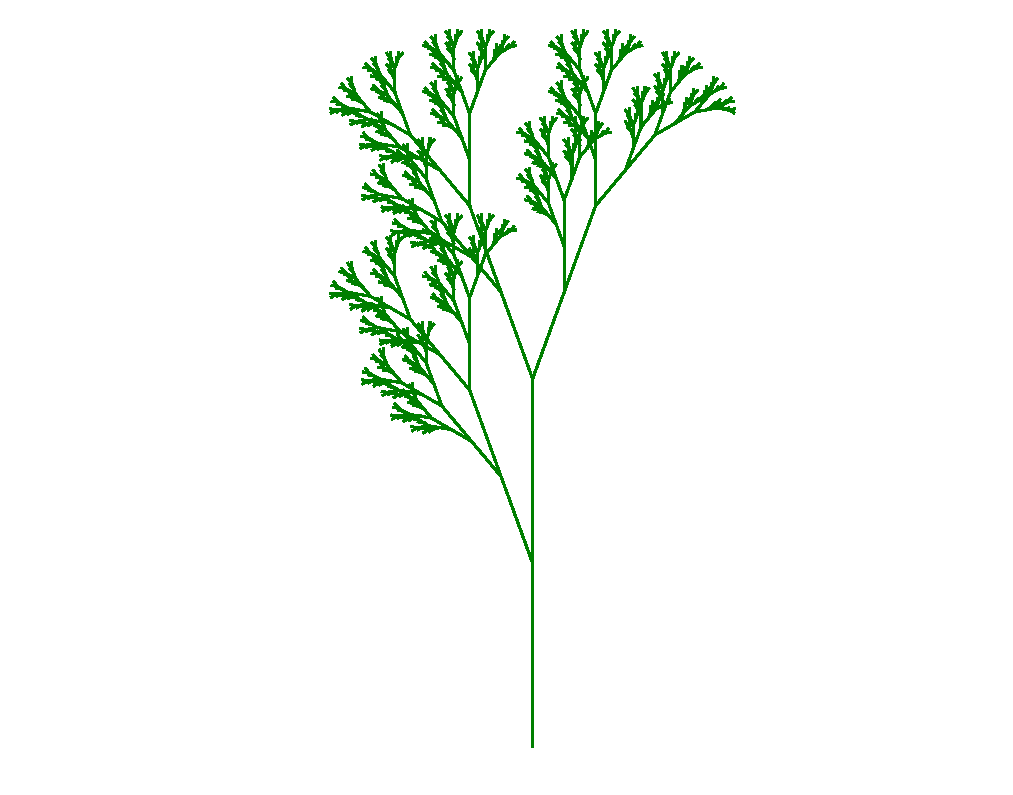
\includegraphics[width=4cm]{Creecriture_4_fig.pdf}
    \caption{Exple 1: 7 itér.}
    \label{fig:Creecriture_4}
  \end{subfigure}
  \begin{subfigure}[b]{4cm}
    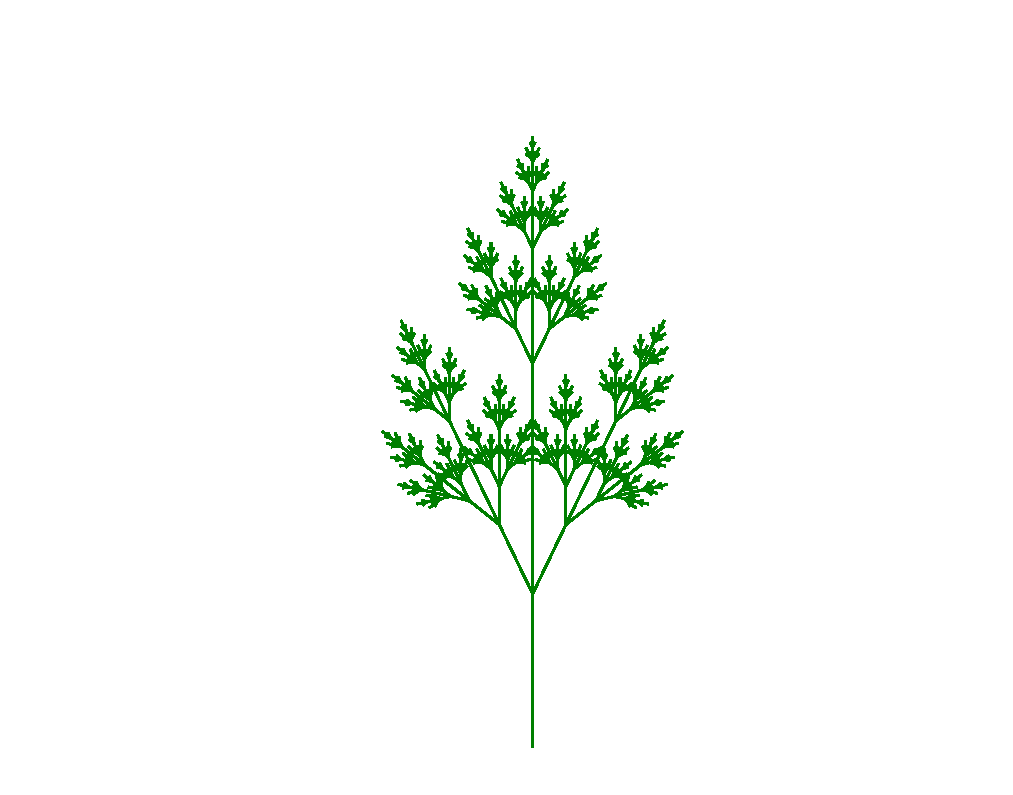
\includegraphics[width=4cm]{Creecriture_5_fig.pdf}
    \caption{Exple 2: 7 itér.}
    \label{fig:Creecriture_5}
  \end{subfigure}
  \begin{subfigure}[b]{4cm}
    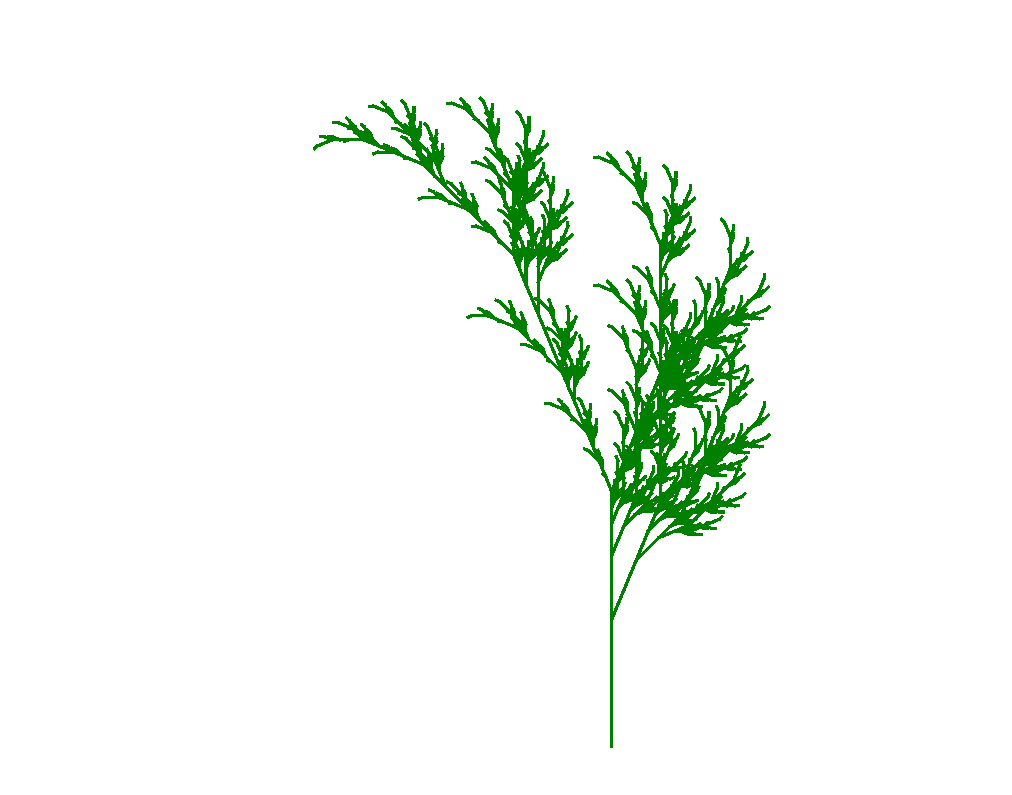
\includegraphics[width=4cm]{Creecriture_6_fig.pdf}
    \caption{Exple 3: 6 itér.}
    \label{fig:Creecriture_6}
  \end{subfigure}
  \caption{Modèles avec apex}
\end{figure}

